\documentclass[11pt,]{article}
\usepackage[]{mathpazo}
\usepackage{amssymb,amsmath}
\usepackage{ifxetex,ifluatex}
\usepackage{fixltx2e} % provides \textsubscript
\ifnum 0\ifxetex 1\fi\ifluatex 1\fi=0 % if pdftex
  \usepackage[T1]{fontenc}
  \usepackage[utf8]{inputenc}
\else % if luatex or xelatex
  \ifxetex
    \usepackage{mathspec}
  \else
    \usepackage{fontspec}
  \fi
  \defaultfontfeatures{Ligatures=TeX,Scale=MatchLowercase}
\fi
% use upquote if available, for straight quotes in verbatim environments
\IfFileExists{upquote.sty}{\usepackage{upquote}}{}
% use microtype if available
\IfFileExists{microtype.sty}{%
\usepackage{microtype}
\UseMicrotypeSet[protrusion]{basicmath} % disable protrusion for tt fonts
}{}
\usepackage[margin=1in]{geometry}
\usepackage{hyperref}
\hypersetup{unicode=true,
            pdftitle={R Markdown Demo PDF},
            pdfauthor={Julia Clark},
            pdfborder={0 0 0},
            breaklinks=true}
\urlstyle{same}  % don't use monospace font for urls
\usepackage{natbib}
\bibliographystyle{apsr}
\usepackage{color}
\usepackage{fancyvrb}
\newcommand{\VerbBar}{|}
\newcommand{\VERB}{\Verb[commandchars=\\\{\}]}
\DefineVerbatimEnvironment{Highlighting}{Verbatim}{commandchars=\\\{\}}
% Add ',fontsize=\small' for more characters per line
\usepackage{framed}
\definecolor{shadecolor}{RGB}{248,248,248}
\newenvironment{Shaded}{\begin{snugshade}}{\end{snugshade}}
\newcommand{\AlertTok}[1]{\textcolor[rgb]{0.94,0.16,0.16}{#1}}
\newcommand{\AnnotationTok}[1]{\textcolor[rgb]{0.56,0.35,0.01}{\textbf{\textit{#1}}}}
\newcommand{\AttributeTok}[1]{\textcolor[rgb]{0.77,0.63,0.00}{#1}}
\newcommand{\BaseNTok}[1]{\textcolor[rgb]{0.00,0.00,0.81}{#1}}
\newcommand{\BuiltInTok}[1]{#1}
\newcommand{\CharTok}[1]{\textcolor[rgb]{0.31,0.60,0.02}{#1}}
\newcommand{\CommentTok}[1]{\textcolor[rgb]{0.56,0.35,0.01}{\textit{#1}}}
\newcommand{\CommentVarTok}[1]{\textcolor[rgb]{0.56,0.35,0.01}{\textbf{\textit{#1}}}}
\newcommand{\ConstantTok}[1]{\textcolor[rgb]{0.00,0.00,0.00}{#1}}
\newcommand{\ControlFlowTok}[1]{\textcolor[rgb]{0.13,0.29,0.53}{\textbf{#1}}}
\newcommand{\DataTypeTok}[1]{\textcolor[rgb]{0.13,0.29,0.53}{#1}}
\newcommand{\DecValTok}[1]{\textcolor[rgb]{0.00,0.00,0.81}{#1}}
\newcommand{\DocumentationTok}[1]{\textcolor[rgb]{0.56,0.35,0.01}{\textbf{\textit{#1}}}}
\newcommand{\ErrorTok}[1]{\textcolor[rgb]{0.64,0.00,0.00}{\textbf{#1}}}
\newcommand{\ExtensionTok}[1]{#1}
\newcommand{\FloatTok}[1]{\textcolor[rgb]{0.00,0.00,0.81}{#1}}
\newcommand{\FunctionTok}[1]{\textcolor[rgb]{0.00,0.00,0.00}{#1}}
\newcommand{\ImportTok}[1]{#1}
\newcommand{\InformationTok}[1]{\textcolor[rgb]{0.56,0.35,0.01}{\textbf{\textit{#1}}}}
\newcommand{\KeywordTok}[1]{\textcolor[rgb]{0.13,0.29,0.53}{\textbf{#1}}}
\newcommand{\NormalTok}[1]{#1}
\newcommand{\OperatorTok}[1]{\textcolor[rgb]{0.81,0.36,0.00}{\textbf{#1}}}
\newcommand{\OtherTok}[1]{\textcolor[rgb]{0.56,0.35,0.01}{#1}}
\newcommand{\PreprocessorTok}[1]{\textcolor[rgb]{0.56,0.35,0.01}{\textit{#1}}}
\newcommand{\RegionMarkerTok}[1]{#1}
\newcommand{\SpecialCharTok}[1]{\textcolor[rgb]{0.00,0.00,0.00}{#1}}
\newcommand{\SpecialStringTok}[1]{\textcolor[rgb]{0.31,0.60,0.02}{#1}}
\newcommand{\StringTok}[1]{\textcolor[rgb]{0.31,0.60,0.02}{#1}}
\newcommand{\VariableTok}[1]{\textcolor[rgb]{0.00,0.00,0.00}{#1}}
\newcommand{\VerbatimStringTok}[1]{\textcolor[rgb]{0.31,0.60,0.02}{#1}}
\newcommand{\WarningTok}[1]{\textcolor[rgb]{0.56,0.35,0.01}{\textbf{\textit{#1}}}}
\usepackage{graphicx,grffile}
\makeatletter
\def\maxwidth{\ifdim\Gin@nat@width>\linewidth\linewidth\else\Gin@nat@width\fi}
\def\maxheight{\ifdim\Gin@nat@height>\textheight\textheight\else\Gin@nat@height\fi}
\makeatother
% Scale images if necessary, so that they will not overflow the page
% margins by default, and it is still possible to overwrite the defaults
% using explicit options in \includegraphics[width, height, ...]{}
\setkeys{Gin}{width=\maxwidth,height=\maxheight,keepaspectratio}
\IfFileExists{parskip.sty}{%
\usepackage{parskip}
}{% else
\setlength{\parindent}{0pt}
\setlength{\parskip}{6pt plus 2pt minus 1pt}
}
\setlength{\emergencystretch}{3em}  % prevent overfull lines
\providecommand{\tightlist}{%
  \setlength{\itemsep}{0pt}\setlength{\parskip}{0pt}}
\setcounter{secnumdepth}{5}
% Redefines (sub)paragraphs to behave more like sections
\ifx\paragraph\undefined\else
\let\oldparagraph\paragraph
\renewcommand{\paragraph}[1]{\oldparagraph{#1}\mbox{}}
\fi
\ifx\subparagraph\undefined\else
\let\oldsubparagraph\subparagraph
\renewcommand{\subparagraph}[1]{\oldsubparagraph{#1}\mbox{}}
\fi

%%% Use protect on footnotes to avoid problems with footnotes in titles
\let\rmarkdownfootnote\footnote%
\def\footnote{\protect\rmarkdownfootnote}

%%% Change title format to be more compact
\usepackage{titling}

% Create subtitle command for use in maketitle
\newcommand{\subtitle}[1]{
  \posttitle{
    \begin{center}\large#1\end{center}
    }
}

\setlength{\droptitle}{-2em}

  \title{R Markdown Demo PDF}
    \pretitle{\vspace{\droptitle}\centering\huge}
  \posttitle{\par}
  \subtitle{Based on `RMarkdownPDFExample.Rmd' by Garret Christensen}
  \author{Julia Clark}
    \preauthor{\centering\large\emph}
  \postauthor{\par}
      \predate{\centering\large\emph}
  \postdate{\par}
    \date{22 April, 2019}

\usepackage[english]{babel}
\usepackage{color}
\usepackage{float}
\usepackage{hyperref}
\hypersetup{colorlinks, linkcolor=, urlcolor=blue, citecolor=blue}
\setlength\parindent{0pt}
\setlength\parskip{0.12in}
\frenchspacing

\begin{document}
\maketitle
\begin{abstract}
If I were writing an article and had an abstract, it would go here!
\end{abstract}

\hypertarget{what-is-r-markdown}{%
\section{What is R Markdown?}\label{what-is-r-markdown}}

This is an R Markdown document. Markdown is a simple formatting syntax
for reports with embedded R code that can be exported as an html, pdf,
MS Word, ODT, RTF, or markdown document; or as an html or pdf-based
(Beamer) slide show.

Essentially, you write a document---like this one---in RStudio using
Markdown syntax. Then you embed chunks of R code in the document, like
this:

\begin{Shaded}
\begin{Highlighting}[]
\KeywordTok{summary}\NormalTok{(iris)}
\end{Highlighting}
\end{Shaded}

\begin{verbatim}
##   Sepal.Length    Sepal.Width     Petal.Length    Petal.Width   
##  Min.   :4.300   Min.   :2.000   Min.   :1.000   Min.   :0.100  
##  1st Qu.:5.100   1st Qu.:2.800   1st Qu.:1.600   1st Qu.:0.300  
##  Median :5.800   Median :3.000   Median :4.350   Median :1.300  
##  Mean   :5.843   Mean   :3.057   Mean   :3.758   Mean   :1.199  
##  3rd Qu.:6.400   3rd Qu.:3.300   3rd Qu.:5.100   3rd Qu.:1.800  
##  Max.   :7.900   Max.   :4.400   Max.   :6.900   Max.   :2.500  
##        Species  
##  setosa    :50  
##  versicolor:50  
##  virginica :50  
##                 
##                 
## 
\end{verbatim}

When you click the \textbf{Knit} button, a document (e.g., HTML, PDF)
will be generated that includes the content you've typed as well as the
output of any embedded R code chunks within the document.

This means that your code, analysis, and output are all in the same
place! You never have to copy-and-paste a table or figure again! If you
change your code and get and estimated effect size of 0.3 instead of
0.5, you don't need to scour your results section or use find and
replace to change this result.

For more details on using R Markdown see
\url{http://rmarkdown.rstudio.com}. Also check out
\href{http://rmarkdown.rstudio.com/lesson-1.html}{this tutorial} and
\href{https://www.rstudio.com/wp-content/uploads/2016/03/rmarkdown-cheatsheet-2.0.pdf}{this
cheatsheet}.

\hypertarget{getting-started}{%
\section{Getting Started}\label{getting-started}}

\hypertarget{installing-and-loading}{%
\subsection{Installing and Loading}\label{installing-and-loading}}

To use R Markdown, you need R and RStudio installed. Let's do that now:

\begin{enumerate}
\def\labelenumi{\arabic{enumi}.}
\tightlist
\item
  Download and install \href{https://cran.rstudio.com/}{R}
\item
  Download and install
  \href{https://www.rstudio.com/products/rstudio/download/}{RStudio}---an
  ``integrated development environment''" or IDE for R
\end{enumerate}

Once you've got \textbf{RStudio open}, then

\begin{enumerate}
\def\labelenumi{\arabic{enumi}.}
\setcounter{enumi}{2}
\tightlist
\item
  Install the R Markdown package by typing
  \texttt{install.packages("rmarkdown")} into the console
\item
  Open a new .Rmd document {[}File \textgreater{} New File
  \textgreater{} R Markdown \ldots{}{]}
\end{enumerate}

\hypertarget{basic-syntax}{%
\subsection{Basic Syntax}\label{basic-syntax}}

The content of an .rdm file is a mixture of different types of syntax
and code, including:

\begin{itemize}
\tightlist
\item
  An (optional) YAML header at the beginning surrounded by
  ``\texttt{-\/-\/-}''---this header gives basic document metadata and
  sets key style and other options, as desired
\item
  Text using Markdown formatting---like this!
\item
  R code chunks, which are the same bits of code you would write in a .R
  script file
\item
  \LaTeX~syntax---enclose text in ``\texttt{\$}'' for inline equations,
  e.g., \(\hat \beta = (X'X)^{-1}X'y\) or ``\texttt{\$\$}'' for
  displayed equations: \[\hat \beta = (X'X)^{-1}X'y \]
\end{itemize}

\hypertarget{basic-options}{%
\subsection{Basic Options}\label{basic-options}}

Within the R code cunks, you can se the following options:

\begin{itemize}
\tightlist
\item
  \texttt{echo=FALSE}---prevents R source code from displaying
\item
  \texttt{eval=FALSE}---prevents Knitr from evaluating the R code
\item
  \texttt{results=\textquotesingle{}hide\textquotesingle{}}---hides the
  results of the code
\item
  \texttt{include=FALSE}---Knitr will run the code but not include in
  the final doc
\item
  \texttt{warning=FALSE}---turns off warnings
\item
  \texttt{message=FALSE}---turns off messages
\end{itemize}

\hypertarget{analysis-example}{%
\section{Analysis Example}\label{analysis-example}}

Let's first begin by clearing our workspace and setting our working
directory:

\begin{Shaded}
\begin{Highlighting}[]
\KeywordTok{rm}\NormalTok{(}\DataTypeTok{list =} \KeywordTok{ls}\NormalTok{()) }\CommentTok{# clear workspace; always a good idea when starting}
\CommentTok{#setwd ("~/Documents/RA/India_BITSS/rmarkdown") # change your working directory}
\end{Highlighting}
\end{Shaded}

Then, let's load our packages:

\begin{Shaded}
\begin{Highlighting}[]
\NormalTok{need <-}\StringTok{ }\KeywordTok{c}\NormalTok{(}\StringTok{"foreign"}\NormalTok{, }\StringTok{"sandwich"}\NormalTok{, }\StringTok{"ggplot2"}\NormalTok{, }\StringTok{"stargazer"}\NormalTok{) }\CommentTok{# list packages you need}
\NormalTok{have <-}\StringTok{ }\NormalTok{need }\OperatorTok\StringTok{ }\KeywordTok{rownames}\NormalTok{(}\KeywordTok{installed.packages}\NormalTok{()) }\CommentTok{# see which are already}
\ControlFlowTok{if}\NormalTok{(}\KeywordTok{any}\NormalTok{(}\OperatorTok{!}\NormalTok{have)) }\KeywordTok{install.packages}\NormalTok{(need[}\OperatorTok{!}\NormalTok{have]) }\CommentTok{# installs the missing ones }
\KeywordTok{invisible}\NormalTok{(}\KeywordTok{lapply}\NormalTok{(need, library, }\DataTypeTok{character.only=}\NormalTok{T)) }\CommentTok{# then loads them all}
\end{Highlighting}
\end{Shaded}

Load the data:

\begin{Shaded}
\begin{Highlighting}[]
\NormalTok{washb <-}\StringTok{ }\NormalTok{haven}\OperatorTok{::}\KeywordTok{read_dta}\NormalTok{(}\StringTok{"WASHBpublic_mock.dta"}\NormalTok{)}
\end{Highlighting}
\end{Shaded}

Run the models:

\begin{Shaded}
\begin{Highlighting}[]
\NormalTok{model1 <-}\StringTok{ }\KeywordTok{lm}\NormalTok{(free_chl_yn }\OperatorTok{~}\StringTok{ }\NormalTok{treatw, }\DataTypeTok{data =}\NormalTok{ washb) }
\NormalTok{model2 <-}\StringTok{ }\KeywordTok{lm}\NormalTok{(free_chl_yn }\OperatorTok{~}\StringTok{ }\NormalTok{treatw }\OperatorTok{+}\StringTok{ }\NormalTok{kiswahili }\OperatorTok{+}\StringTok{ }\NormalTok{english, }\DataTypeTok{data =}\NormalTok{ washb)}
\NormalTok{robust.se1 <-}\StringTok{ }\KeywordTok{sqrt}\NormalTok{(}\KeywordTok{diag}\NormalTok{(}\KeywordTok{vcovHC}\NormalTok{(model1, }\DataTypeTok{type =} \StringTok{"HC"}\NormalTok{)))}
\NormalTok{robust.se2 <-}\StringTok{ }\KeywordTok{sqrt}\NormalTok{(}\KeywordTok{diag}\NormalTok{(}\KeywordTok{vcovHC}\NormalTok{(model2, }\DataTypeTok{type =} \StringTok{"HC"}\NormalTok{)))}
\end{Highlighting}
\end{Shaded}

And make our table:

\begin{Shaded}
\begin{Highlighting}[]
\KeywordTok{stargazer}\NormalTok{(model1, model1, }\DataTypeTok{se=}\KeywordTok{list}\NormalTok{(robust.se1, robust.se2), }
          \DataTypeTok{title=}\StringTok{"Made Automatically in R"}\NormalTok{, }
          \DataTypeTok{out=}\StringTok{"outputR.tex"}\NormalTok{, }\DataTypeTok{header=}\OtherTok{FALSE}\NormalTok{)}
\end{Highlighting}
\end{Shaded}

\begin{table}[!htbp] \centering 
  \caption{Made Automatically in R} 
  \label{} 
\begin{tabular}{@{\extracolsep{5pt}}lcc} 
\\[-1.8ex]\hline 
\hline \\[-1.8ex] 
 & \multicolumn{2}{c}{\textit{Dependent variable:}} \\ 
\cline{2-3} 
\\[-1.8ex] & \multicolumn{2}{c}{free\_chl\_yn} \\ 
\\[-1.8ex] & (1) & (2)\\ 
\hline \\[-1.8ex] 
 treatw & 0.364$^{***}$ & 0.364$^{***}$ \\ 
  & (0.043) & (0.043) \\ 
  & & \\ 
 Constant & 0.013 & 0.013 \\ 
  & (0.009) & (0.045) \\ 
  & & \\ 
\hline \\[-1.8ex] 
Observations & 284 & 284 \\ 
R$^{2}$ & 0.223 & 0.223 \\ 
Adjusted R$^{2}$ & 0.220 & 0.220 \\ 
Residual Std. Error (df = 282) & 0.340 & 0.340 \\ 
F Statistic (df = 1; 282) & 81.002$^{***}$ & 81.002$^{***}$ \\ 
\hline 
\hline \\[-1.8ex] 
\textit{Note:}  & \multicolumn{2}{r}{$^{*}$p$<$0.1; $^{**}$p$<$0.05; $^{***}$p$<$0.01} \\ 
\end{tabular} 
\end{table}

Note that we needed the
\texttt{results\ =\ \textquotesingle{}asis\textquotesingle{}} option to
get the table to output correctly, otherwise we would have gotten the
copy-and-paste \LaTeX~output like in R.

\hypertarget{referring-to-values}{%
\subsection{Referring to values}\label{referring-to-values}}

You can refer to values calculated in R by just surrounding ``r'' and
the code with single accent marks. For example, the mean frequency is
0.4822888. The mean frequency rounded to two decimal place is 0.48.

\hypertarget{figuresplots}{%
\section{Figures/Plots}\label{figuresplots}}

For figures generated in R, you can code them directly (here, the data
comes from the \texttt{iris} dataset, which comes pre-loaded in R:

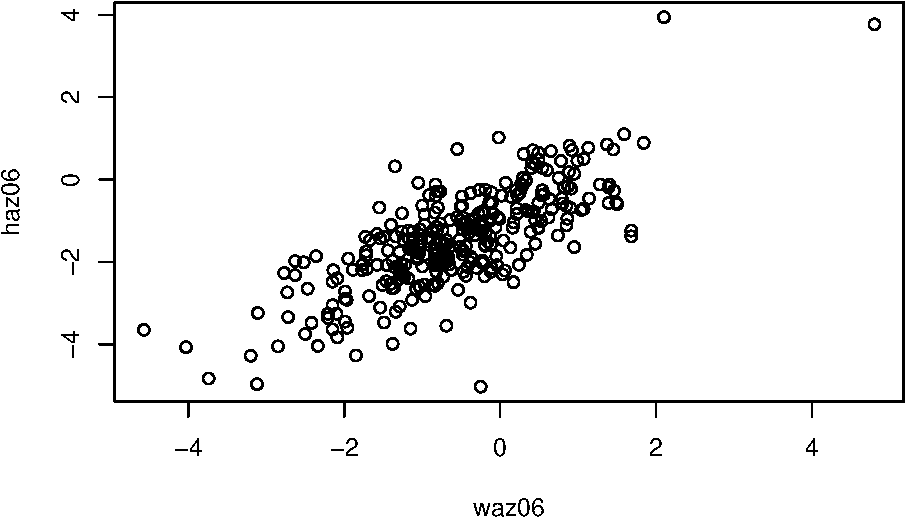
\includegraphics{Rmarkdown_advanced_files/figure-latex/unnamed-chunk-5-1.pdf}

Note that the \texttt{echo\ =\ FALSE} parameter was added to the code
chunk to prevent printing of the R code that generated the plot.

For external files that you want to include, use
\texttt{image:\ !{[}{]}(de-identification\_indirect.png)}. Or you can
use \LaTeX~syntax if you want advanced formatting capacity, e.g.,

\begin{figure}[H]
  \centering
  \caption{Options for De-Identifying Data}
  \includegraphics[width=\textwidth]{de-identification_indirect.png}
\end{figure}

\hypertarget{basic-formatting-in-markdown}{%
\section{Basic Formatting in
Markdown}\label{basic-formatting-in-markdown}}

\hypertarget{headers}{%
\subsection{Headers}\label{headers}}

Make yourself a header of different levels using \texttt{\#} for level
1, \texttt{\#\#} for level 2 etc.

\hypertarget{typeface}{%
\subsection{Typeface}\label{typeface}}

Surround words in \texttt{*} for \emph{italics}, and \texttt{**} for
\textbf{bold}.

\hypertarget{punctuation}{%
\subsection{Punctuation}\label{punctuation}}

Use ``\texttt{-\/-\/-}''" to get an em-dash (---) and ``\texttt{-\/-}''"
to get an en-dash (--). Use normal quotation marks ("", or ''), unlike
in \LaTeX.

\hypertarget{lists}{%
\subsection{Lists}\label{lists}}

Make a numbered list using ``\texttt{1.}'', and a bulleted list using
``\texttt{-}'':

\begin{enumerate}
\def\labelenumi{\arabic{enumi}.}
\tightlist
\item
  item 1
\item
  item 2
\item
  item 3
\end{enumerate}

\begin{itemize}
\tightlist
\item
  item a
\item
  item b
\item
  item c
\end{itemize}

\hypertarget{hyperlinks}{%
\subsection{Hyperlinks}\label{hyperlinks}}

Rmarkdown will automatically format a copy-and-pasted URL as a hyperlink
(e.g., \url{http://rmarkdown.rstudio.com}). If you want to add a link to
a particular word, type
``\texttt{{[}Rstudio{]}(http://rmarkdown.rstudio.com)}'' to get
\href{http://rmarkdown.rstudio.com}{Rstudio}.

\hypertarget{commenting}), and markdown
(\texttt{\textless{}!-\/-\ -\/-\textgreater{}}). In the preamble and
code snippets, comment using \texttt{\#} as in R (see above). In the
rest of the document, comment by surrounding text with
\texttt{\textless{}!-\/-\ -\/-\textgreater{}}.

\hypertarget{footnotes-and-citations}{%
\section{Footnotes and Citations}\label{footnotes-and-citations}}

\hypertarget{footnotes}{%
\subsection{Footnotes}\label{footnotes}}

Add a footnote using \texttt{\^{}{[}I\ am\ a\ footnote{]}}.\footnote{I
  am a footnote.}

\hypertarget{citations}{%
\subsection{Citations}\label{citations}}

Here's how you add a citation from your BibTex library (formatted in
author-date style, using the \texttt{natbib} package loaded in the
preamble):

\begin{itemize}
\tightlist
\item
  For a single source, use \texttt{{[}@citekey{]}}, e.g.,
  ``\texttt{{[}@banerjee2010pitfalls{]}}'' gives us
  \citep{banerjee2010pitfalls}.
\item
  For multiple sources, use \texttt{{[}@citekey1;\ @citekey2;\ etc.{]}},
  e.g., ``\texttt{{[}@banerjee2010pitfalls;\ @easterly2001elusive{]}}''
  gives us \citep{banerjee2010pitfalls, easterly2001elusive}.
\item
  For an in-text citation, use \texttt{@citekey} with no brackets, e.g.,
  ``\texttt{@banerjee2010pitfalls}'' gives us
  \citet{banerjee2010pitfalls}.
\end{itemize}

For more, see
\url{http://rmarkdown.rstudio.com/authoring_bibliographies_and_citations.html}.

And the bibliography/references will automatically show up with the
sources you've added using cite keys; no need to copy and paste
citations or double check to make sure you've included/removed sources
as necessary!\ldots{}

\bibliography{my\_bib.bib}


\end{document}
